\documentclass[9pt]{beamer}
\usepackage{xeCJK}
\usepackage[space,space,hyperref]{ctex}
\setsansfont{Ubuntu Mono}
\usefonttheme[onlymath]{serif}
\setCJKmonofont{AR PL UKai CN}
\usetheme{metropolis}
\title{水题选讲}
\date{\today}
\author{雅礼中学高二信息组}
\begin{document}

  \maketitle
\begin{frame}{作为今天的开胃小水题}
	今天来讲一个经典题\pause
	的加强版。

	\pause
	可能有人见过了,不过放在联赛题目的宣讲小清新开场还不错。
\end{frame}
\section{某题}
\begin{frame}{Statement}
	给定一棵大小为$n$的有标号无根树和一参数$k$。
	
	求有几棵同样大小为$n$的树的边集的与原树边集的交集大小不小于$k$。

	经典范围:$n\le 100$

	加强范围:$n\le 5000$
\end{frame}
\section{naive solution}
\begin{frame}{$n\le 100$}
	考虑矩阵树定理。

	对大小为$n$的完全图运用矩阵树定理:把原树中出现的边权设为$x$,其他的边设为$1$。\pause

	容易发现,求出的行列式是一个关于$x$的多项式$f(x)$,求出$\sum_{i\geq k}[x^i]f(x)$即可。

	暴力求$f(x)$也不难,枚举点值然后插值就行了。\pause

	$\mathcal O(n^4)$
\end{frame}
\section{better solution}
\begin{frame}{$n \le 5000$}
	矩阵树定理好像没啥前途。\pause

	如果我们现在已经钦定了一些边一定相同(即一定出现在交集中),怎么统计方案呢?

	现在我们面临的局面是:有$n$个点形成了$k$个连通块,第$i$个连通块的大小为$s_i$,求把它们连成一棵树的方案数。\pause

	朋友,你看过\href{https://oi-wiki.org/graph/prufer/}{oi-wiki上介绍prufer的页面吗}?

	\begin{center}
		
\includegraphics[width=10cm]{prufer-query.png}

		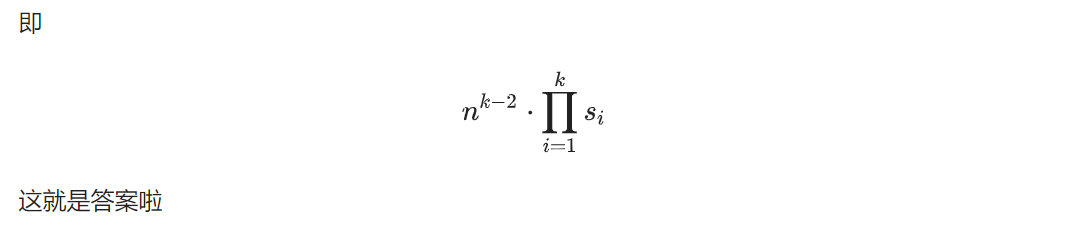
\includegraphics[width=10cm]{prufer-answer.png}
	\end{center}
	\pause

	具体证明可以考虑枚举prufer序列,oi-wiki上讲解得非常详细,不再赘述。
\end{frame}
\begin{frame}{$n \le 5000$}
	所以我们现在面临的问题变成了:求所有钦定$m$条边相同时,$\prod a_i$的和。
	\pause
	
	朋友,你听说过WC[2019]数树吗?

	$a_i$的组合意义也就是“在$i$号连通块里面选出一个点。”
	\pause

	好做了,设$f_{u,l,0/1}$表示“$u$的子树内钦定$l$条边相同,当前连通块选不选点”的方案数,dp即可。

	最后再套一个二项式反演就行啦。\pause

	$\mathcal O(n^2)$
\end{frame}

  \section{CF Gym 102576 D}
  \begin{frame}{CF Gym 102576 D}
    \onslide<1-> 题意:给出一个圆的 $n$ 条圆弧,求一个最大的子集满足子集中的圆弧两两有交。$1\le n \le 3000$ 。
  \end{frame}
  \begin{frame}{CF Gym 102576 D}
    \onslide<1-> 由于是在圆上,所以选取的圆弧之间可能没有共同的弧。
    \begin{center}
      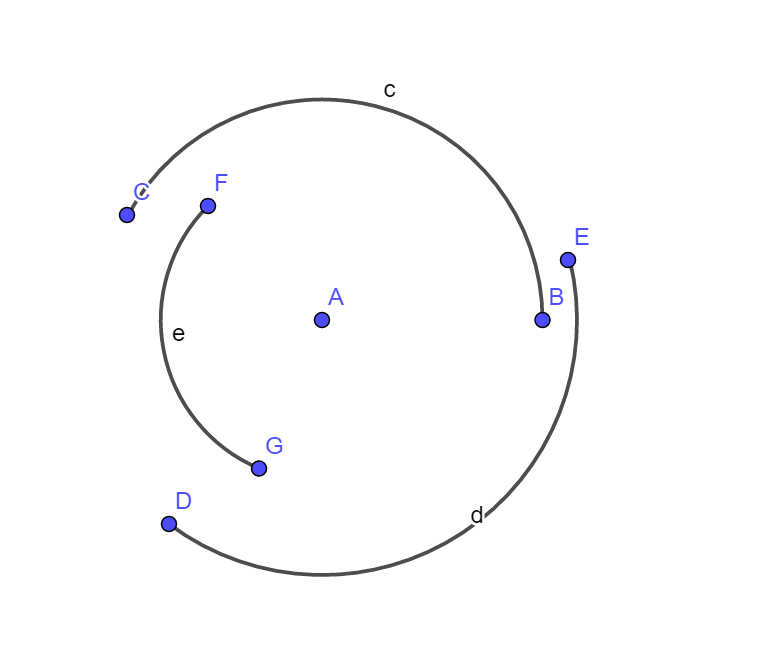
\includegraphics[width=5cm]{photo1.png}
    \end{center}

    \onslide<2-> 考虑钦定一条圆弧必须选,且不能选取被它完全包含的圆弧。

    \onslide<3-> 这样的话,能被选中的其它弧显然与该弧的左右端点有交。

    \onslide<4-> 那么,完全包含它的以及与它两端都相交的显然可以选,与它相离的显然不选。

    \onslide<5-> 于是现在只剩下 $2$ 种候选的圆弧(与选取弧的左端相交或右端相交)需要讨论了。
  \end{frame}
  \begin{frame}{CF Gym 102576 D}
    \onslide<1-> 我们令与左端相交的弧为 $A$ 类弧,与右端相交的弧为 $B$ 类弧,以选取弧为参照物,考虑它们相交的条件。
    \begin{center}
      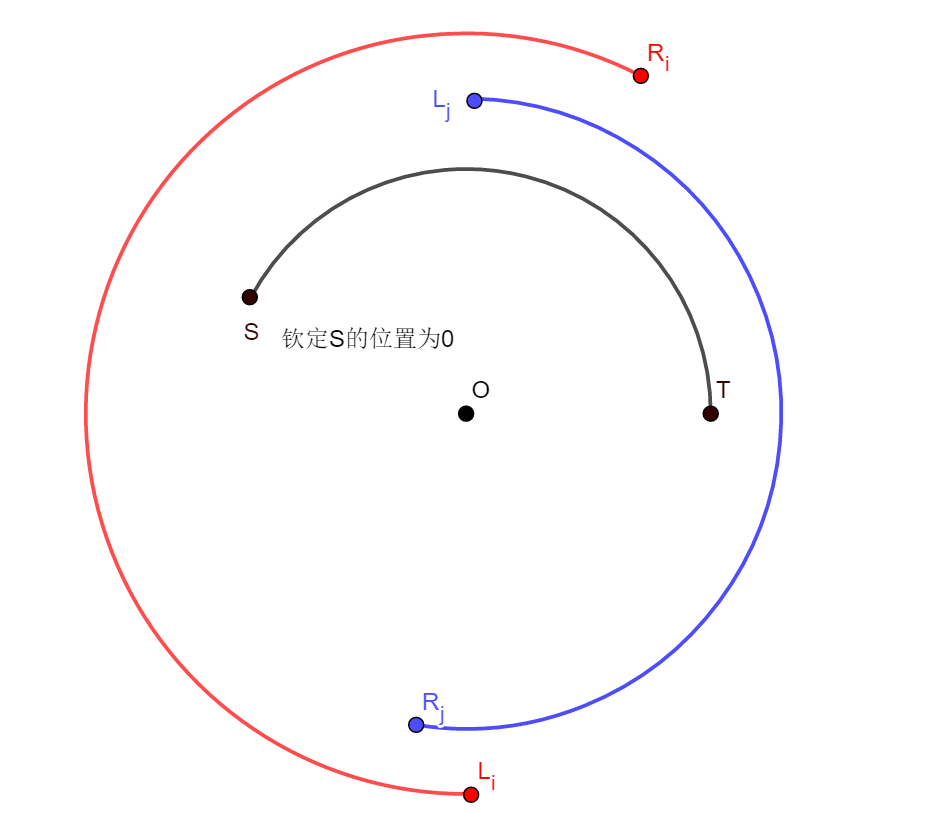
\includegraphics[width=5cm]{photo2.png}
    \end{center}

    \onslide<2-> 一个非常好的性质是, $A$ 类弧都满足 $L_i\ge R_i$,$B$ 类弧都满足 $L_j\le R_j$。

    \onslide<3-> 假设 $A$ 类弧为 $i$,$B$ 类弧为 $j$ ,那么它们相交的充要条件是$ R_i\ge L_j$ 或 $L_i\le R_j$ 。
  \end{frame}
  \begin{frame}{CF Gym 102576 D}
    \onslide<1-> 不难发现可以转化为在二维平面上的数点问题,令 $A$ 类弧为黑点$(R_i,L_i)$, $B$ 类弧为白点$(L_j,R_j)$,那么限制就是黑点不能在白点左上方,如图:
    \begin{center}
      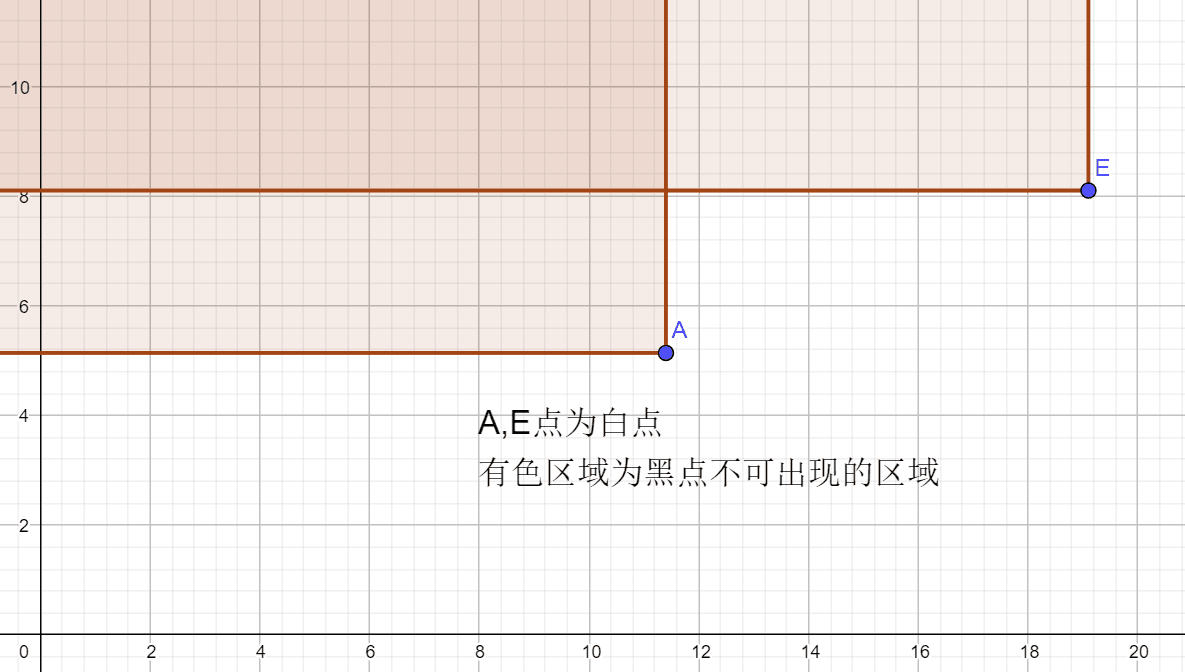
\includegraphics[width=5cm]{photo3.png}
    \end{center}
  
  ​	\onslide<2-> 可以用线段树优化DP转移。时间复杂度$O(n^2\log n)$。
  \end{frame}

  \section{CF1386G}
  \begin{frame}{CF1368G}
    \par 在 $n\times m$ 的方格里,用 $1\times2$ 的多米诺骨牌\textbf{恰好}填满。
    \par 拿走其中任意一个骨牌,然后可以让任意骨牌以平行于原来的方向移动,但不能转弯。要求一个骨牌最终的位置与初始位置至少有一个格子重合。
    \par 试求出所有空格位置无序二元组的数量。
    \par $n\times m\le200000$ 
  \end{frame}

  \begin{frame}{CF1368G}
    \onslide<1-> 考虑到骨牌移动就是空格的移动。

    \onslide<2-> 考察一个横着的骨牌,$(i,j)$ 与 $(i,j+1)$,那么考虑向左移,空格从 $(i,j-1)$ 到 $(i,j+1)$ ;向右移,空格从 $(i,j+2)$ 到 $(i,j)$ 。竖着的骨牌亦然。

    \onslide<3-> 按照上述空格转移的方式连出若干条边之后,会形成一张图,且每个点入度为 $1$ 。
  \end{frame}

  \begin{frame}{CF1368G}
    \onslide<1-> conclusion 1:

    \onslide<2-> 形成的图无环。

    \onslide<3-> proof 1:

    \onslide<4-> 假设最后形成了一个环。我们一定可以通过多次将任意一个角翻折,使得最终的环围成了一个矩形。

    \onslide<5-> 易知,翻折不会改变矩形内点的奇偶性。又因为特殊的连边方式,矩形的边长都是奇数。

    \onslide<6-> 那么,这个矩形内是无法用骨牌恰好填满的。所以矛盾。

    \onslide<7-> conclusion 2:
    
    \onslide<8-> 如果两个点属于同一个骨牌,那么它们一定不属于同一个弱联通分量。

    \onslide<9-> proof 2:

    \onslide<10-> 考虑到一条边连接的两个点,横纵坐标之和奇偶性不变。则该结论显然。
  \end{frame}
  
  \begin{frame}{CF1368G}
    \onslide<1-> 考虑到两个空格位置 $(x_1,y_1)$ 与 $(x_2,y_2)$ ,能产生贡献的充要条件是,在它们所属的两棵树里,由它们到根的路径中,分别存在两个属于同一骨牌的点。
  
    \onslide<2-> 换言之,一对同一骨牌的点,可以覆盖到它们的两棵子树的点对应形成的点对。

    \onslide<3-> 那么,求出 $dfn$ 之后,相当于在平面上求面积并。这是一道扫描线的经典问题。

    \onslide<4-> 复杂度 $O(nm\log nm)$ 。
  \end{frame}

  \section{CF Gym 100959 K}
  \begin{frame}{CF Gym 100959 K}
    \par 给定一个二维平面上的 $n$ 个黑点,剩下的均为白点,问你最少染多少个点变为黑点可以形成一个正方形网格。一个 $K\times K$ 的正方形网格指,有实数 $a,b,c,d$ 使得 $\forall i,j\in[0,K)\cap Z$ 有 $(a+ci+dj,b+di-cj)$ 为黑点。 
    \par $n\leq 10^5$,二维平面坐标在 $int$ 范围内。
  \end{frame}

  \begin{frame}{CF Gym 100959 K}
    \onslide<1-> 将限制转化后变为: 选定一对基底 $\vec{r_1}, \vec{r_2}$ 和一个原点,使得所有黑点可以在这个原点下,被这个基底用整数系数线性组合

    \onslide<2-> 平凡的,$\vec{r_1}=(1,0),\vec{r_2}=(0,1)$ 一定是一个合法解,但是我们还需要加入的黑点最少。仔细思考可以发现,在基底模长最长的情况下,$K$ 最小
  
    \onslide<3-> 设给定的所有点有 $\vec{v_i}=(a_i,b_i)$ ,则一个满足条件的基底,当且仅当 $\forall i\not= j$ 有 $\vec{v_i}-\vec{v_j}$ 可以被这个基底用整数系数线性组合。由线性代数知识可知,我们只需要满足 $\forall i\in[1,n-1]$ 有 $\vec{v_i}-\vec{v_{i+1}}$ 可以被组合出来即可

    \onslide<4-> 所以问题转化为了给定 $n$ 个向量 $\vec{w_i}$ ,求一个模长最长的基底可以组合出所有 $\vec{w_i}$ 
  \end{frame}

  \begin{frame}{CF Gym 100959 K}
    \onslide<1-> 再由线性代数知识可以得到,如果我们求解出前 $i$ 个向量的最长合法基底 $\vec{r_1},\vec{r_2}$ ,那么只要可以求解出 $\vec{w_{i+1}},\vec{r_1},\vec{r_2}$ 的最长合法基底。而且稍加计算既可发现,若一个基底可以组合出 $(s,t)$ ,那么一定可以组合出 $(t,-s)$ ,所以问题再次化简为求解出 $\vec{w_{i+1}},\vec{r_1}$ 的最长合法基底

    \onslide<2-> 简化一下记号,即求 $\vec{a},\vec{b}$ 的最长合法基底。首先给出做法如下:

    \onslide<3-> 
    \begin{itemize}
      \item 取两者中模长较长的为 $\vec{a}$ ,较短的为 $\vec{b}$ ,令 $\vec{c}$ 为 $\vec{b}$ 的四个方向向量中的任意一个
      \item 若 $\vec{a}-\vec{c}$ 的模长小于 $\vec{a}$ 的模长,$\vec{a}=\vec{a}-\vec{c}$
      \item 若 $\vec{a}$ 的模长等于 $0$ ,则 $b$ 即为所求基底,否则解决这个子问题
    \end{itemize}

    \onslide<4-> 现在需要说明的是,按照这个操作,每次一定可以使 $\vec{a}$ 的模长减小
  \end{frame}

  \begin{frame}{CF Gym 100959 K}
    \onslide<1-> 考虑将 $\vec{b}$ 旋转后建立平面直角坐标系,令 $\vec{c}$ 在 $x,y$ 轴上,假设当前 $\vec{c}$ 为 $x$ 正半轴的基底

    \onslide<2-> 那么做 $\vec{c}$ 的垂直平分线,若 $\vec{a}$ 的垂直平分线的右侧,则 $\vec{a}-\vec{c}$ 的模长一定小于 $\vec{a}$ 的模长

    \onslide<3-> 发现,四条垂直平分线覆盖了包含原点的一个边长为 $|\vec{c}|$ 的小正方形外的所有向量,也就是说,我们每次操作可以试 $\vec{a}$ 的模长变为 $\leq \frac{|\vec{c}|}{2}$ 。因此,一定可以试 $\vec{a}$ 的模长减小,且该操作的运行次数为 $log$ 次

    \onslide<4-> 当我们求得基底后,得到 $\forall i\in[2,n]$ 中,$\vec{a_i}-\vec{a_1}=x_i\vec{r_1}+y_i\vec{r_2}$ ,那么 $K=max\{maxx_i-minx_i,maxy_i-miny_i\}+1$ 
  \end{frame}

  \section{UOJ312 梦中的题面}
  \begin{frame}{UOJ312 梦中的题面}
    \par 题目大意:给定$n,m,b,c$,求出满足以下条件的$m$元组$(x_1,x_2,...,x_m)$的个数
    \par $x_i \in Z$,$0\leqslant x_i \leqslant b^{i}-c$,$x_1+x_2+...+x_m \leqslant n$
    \par 数据范围:$c\in{0,1}$,$0\leqslant n < b^{m+1}$,$2 \leqslant b \leqslant 50$,$1 \leqslant m \leqslant 50$
  \end{frame}
  
  \begin{frame}{UOJ312 梦中的题面}
    \onslide <1-> 这是一道数位$dp$。
    
    \onslide <2-> 先考虑$c=1$的情况,那么我们发现,$x_i$在$b$进制下能且仅能为小于等于$i$位的数。
    
    \onslide <3-> 也就是说,从低到高第$k$位有$k-1$个数这一位只能为$0$,其他数可以取到$0\sim b-1$中的任意值。
    
    \onslide <4-> 预处理一个数组$g_{i,j}$表示$i$个取$0\sim b-1$的数的和恰好为$j$的方案数,从低到高,以所有数的和在这一位的和为状态数位dp并处理进位情况,这一位的和是$O(m+k)$的,直接枚举当前加的数并转移到下一位即可。
  \end{frame}
    
  \begin{frame}{UOJ312 梦中的题面}
    \onslide <1-> 然后是$c=0$的情况。
    
    \onslide <2-> 这时$x_i$可以恰好可以取$b^i$,即在$i+1$位为$1$,并且在其他位时它都为$0$。
    
    \onslide <3-> 可以沿用之前的思路,再加一维表示当前有多少个数必须取$0$,初始时显然个数是任意的。
    
    \onslide <4-> 转移到第$i$位时,判断$x_i$是否取到$b^i$,如果是,那么它之前为$0$且之后也会为$0$,$0$的个数就不变,否则就要加$1$。
    
    \onslide <5-> 那么你就在$O(m^3b^2)$的复杂度内解决了所有情况。
  \end{frame}
    
  \begin{frame}{UOJ312 梦中的题面}
    \onslide <1-> 还可以继续优化。
    
    \onslide <2-> 我们尝试从高位往低位限制这些数的和。
    
    \onslide <3-> 现在记录的就是$n$的高位值减去$dp$的数的高位值
    
    \onslide <4-> 发现这个值大于$m$时,接下来转移的数无论多大都不会使总和达到$n$。
    
    \onslide <5-> 沿用之前的方法,枚举下一位的值转移就可以$O(m^2b^2)$了,很神奇。
  \end{frame}

  \section{CF1208G Polygons}
  \begin{frame}
		\frametitle{CF1208G Polygons}
		\par 给定$n,k$
		\par 你需要构造$k$个有相同外接圆的正多边形,使得边数在$3\sim n$间且边数两两不同
		\par 你可以任意旋转它们,求它们与这个外接圆的最少交点数
		\par $k\le n-2,n\le 10^6$
	\end{frame}
	\clearpage
	\begin{frame}
		\frametitle{solution}
		\onslide<1-> 显然,这些多边形会有一个共同的交点

		\onslide<2-> 于是,发现如果$u|v$,那么$u$肯定比$v$先选

		\onslide<3-> 并且如果所有$u|v$都选了,那么$v$的代价为$\phi(v)$

		\onslide<4-> 按$\phi$排序后从小到大选即可,当然因为没有$2$边形,特判掉即可
	\end{frame}
	\clearpage
	\clearpage
	\begin{frame}
		\frametitle{end}
		\onslide<1-> 本次讲课作为一道noip难度的讲课

		\onslide<2-> 覆盖面广

		\onslide<3-> 难度适中

		\onslide<4-> 题量适中

		\onslide<5-> 解法自然

		\onslide<6-> 讲课人相信,这次美妙的讲课,可以给即将AK[[CSP|NOIP]2020|[联合省选|NOI]2021|[WC|CTS|IOI]2022]的你,提供一个有力的帮助
	\end{frame}

  \section{Thanks}

\end{document}
